\section{实变量的凸函数}

设 H 是 R 的一个子集，f 是定义在 H 上的有限实函数，设 G 是函数 f 在 \(R \times R = R^{2}\) 中的图像（或表示集），即点 \(M_{x} = (x, f(x))\) 所成的集，其中 x 跑遍 H。方便起见，我们说：点 \((a, b)\) （\(R^{2}\) 中的，满足 \(a \in H\) ）位于 G 之上（相应地，严格位于 G 之上、位于 G 之下、严格位于 G 之下），如果有 \(b \geqslant f(a)\) （相应地，\(b > f(a), b \leqslant f(a), b < f(a)\) ）。若 \(A = (a, a')\) 与 \(B = (b, b')\) 是 \(R^{2}\) 中两点，我们用 AB 表示以 A 与 B 为端点的闭线段；若 a \textless{} b，则 AB 是线性函数 \(a' + \frac{b' - a'}{b - a} (x - a)\) （定义在 {[}a, b{]} 上的）的图像；我们把该线段的斜率 \(\frac{b' - a'}{b - a}\) 记作 \(p(\text{AB})\) ，并将使用下面这个引理，其验证是直接的：

引理. 设 \(\mathrm{A} = (a, a')\) 、\(\mathrm{B} = (b, b')\) 、\(\mathrm{C} = (c, c')\) 是 \(\mathbf{R}^2\) 中三点，满足 \(a < b < c\) 。下列命题等价：

\begin{enumerate}
\def\labelenumi{\alph{enumi})}
\item
  B 位于 AC 之下；
\item
  C 位于过 A 与 B 的直线上方；
\item
  A 位于过 B 与 C 的直线上方；
\item
  \(p(\mathrm{AB}) \leqslant p(\mathrm{AC});\)
\item
  \(p(\mathrm{AC}) \leqslant p(\mathrm{BC})\) .
\end{enumerate}

当把“位于…之上”（相应地，“位于…之下”）换成“严格位于…之上”（相应地，“严格位于…之下”），并把记号 \(\leqslant\) 换成 \textless{} 时，引理仍然成立（fig.~1）。

\pandocbounded{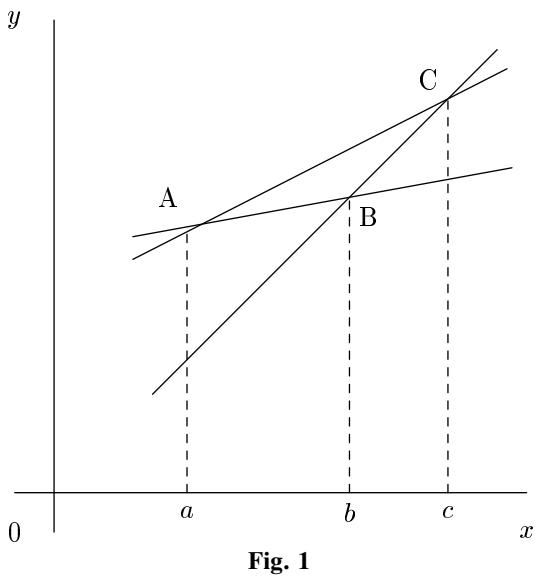
\includegraphics[keepaspectratio]{images/part001_7b60909a.jpg}}

